\chapter{Diseño y desarrollo del juego}\label{sec:desarrollo}

El objetivo principal del proyecto, desde el punto de vista técnico, es el desarrollo de un videojuego para la Game Boy Advance usando el menor número posible de librerías externas. Forzando así un mayor entendimiento de cómo funciona el dispositivo junto con la lógica requerida para poder hacer ciertas funciones aunque ya se proporcionen en la mayoría de librerías existentes para la consola.

Completadas las dos primeras tareas de la planificación, el estudio de la arquitectura y de técnicas de programación, se decide implantar una visión para el proyecto. Para ello, el autor revisita juegos de su agrado en los que basar el proyecto.

Una vez finalizado el proceso de búsqueda de inspiración, la idea inicial del proyecto fue la de recrear las mecánicas y jugabilidad del popular juego de PC \textit{Nidhogg} (véase la Figura~\ref{fig:nidhogg}).

\begin{figure}[h]
	\centering
	
\includegraphics[width=.5\textwidth]{capitulos/capitulo5/nidhogg.jpg}
	\caption{Nidhogg, un juego para ordenador.}\label{fig:nidhogg}
\end{figure}
\FloatBarrier{}

El autor empezó a diseñar los \textit{assets} del juego recreándolos en \textit{Pixelorama}, tal y como se muestra en la Figura~\ref{fig:proto_1}.

\begin{figure}[h]
	\centering
	
\includegraphics[width=.6\textwidth]{capitulos/capitulo5/proto_1.png}
	\caption{\textit{Assets} para el primer prototipo del juego.}\label{fig:proto_1}
\end{figure}
\FloatBarrier{}

Sin embargo, al finalizar la primera iteración se observaron los siguientes riesgos que afectaban el desarrollo del juego:

\begin{itemize}
	\item Multijugador: Una de las fortalezas del juego original fue la posibilidad de conectar con otros jugadores y competir a través de la red, o en la propia máquina con múltiples mandos. Una implementación equivalente tendría que hacer uso de la comunicación serial que ofrece la consola, funcionalidad que dificulta probar el juego en hardware y que la mayoría de emuladores no soporta completamente, ya sea de forma local o en red. En la Figura~\ref{fig:mgba_serial_status} se muestra el estado actual de dicha funcionalidad en el emulador mGBA.

		\begin{figure}[h]
			\centering
			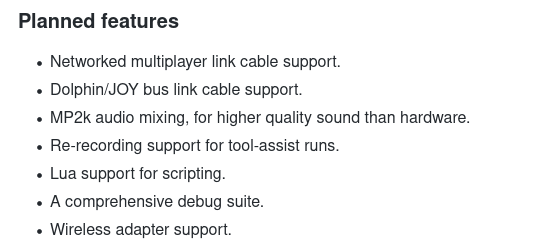
\includegraphics[width=.5\textwidth]{capitulos/capitulo5/mgba_serial_status.png}
			\caption{Funcionalidades por implementar.}\label{fig:mgba_serial_status}
		\end{figure}
		\FloatBarrier{}

	\item Arte: Otro error que se cometió en las primeras fases de desarrollo fue subestimar el tiempo requerido para crear los recursos o \textit{assets} del juego. Por este motivo, el autor decidió hacer uso de recursos \textit{open source} creados por la comunidad, utilizándolos siempre según las condiciones de las licencias utilizadas.
\end{itemize}

Habiendo reevaluado proyecto, se optó por realizar un juego de plataformas. El diseño giraría en torno a un personaje con diversas habilidades, siendo necesario familiarizarse con cada una de ellas para poder superar el juego.

En la segunda iteración se prototiparía un juego medieval (véase la Figura~\ref{fig:proto_2}) utilizando los \textit{assets} creados por \textit{Dagon}\footnote{https://im-dagon.itch.io/dungeon-pack} y acorde con las características descritas previamente. Sin embargo, antes de comenzar con el tercer sprint, se descartaría el diseño al no convencer al autor del proyecto.

\begin{figure}[h]
	\centering
	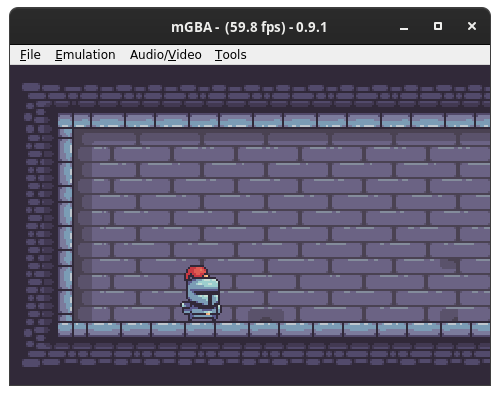
\includegraphics[width=.5\textwidth]{capitulos/capitulo5/proto_2.png}
	\caption{Segundo prototipo del juego.}\label{fig:proto_2}
\end{figure}
\FloatBarrier{}

Finalmente, a partir del tercer \textit{sprint} se optó por utilizar los \textit{assets} creados por \textit{o\_lobster}\footnote{https://o-lobster.itch.io/platformmetroidvania-pixel-art-asset-pack}. En la Figura~\ref{fig:proto_3} se ve una muestra del conjunto de recursos seleccionado en última instancia.

\begin{figure}[h]
	\centering
	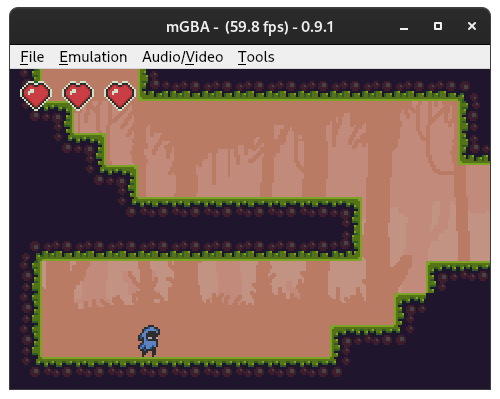
\includegraphics[width=.5\textwidth]{capitulos/capitulo5/preview_lobster.png}
	\caption{Arte escogido para el desarrollo del juego.}\label{fig:proto_3}
\end{figure}
\FloatBarrier{}

A continuación, se detallarán los requisitos y las rutinas utilizadas para poder desarrollar el juego.

\section{Especificaciones}
En esta sección se describe la solución propuesta por el autor para satisfacer las necesidades del juego. La estructura de esta sección se deriva de asignaturas cursadas previamente~\cite{bib:diu}. Los acrónimos que se utilizarán en las próximas secciones son los siguientes:

\begin{itemize}
	\item \textbf{OBJ}: Objetivo (o requisitos generales del juego).
	\item \textbf{PU}: Perfil de Usuario.
	\item \textbf{ACT}: Actor del producto desarrollado.
	\item \textbf{RF}: Requisito Funcional.
	\item \textbf{RI}: Requisito de Información.
	\item \textbf{RNF}: Requisito No Funcional.
\end{itemize}

\subsection{Requisitos generales}
A continuación, se describen los requisitos generales del juego en forma de objetivos.

\begin{table}[h]
	\centering
	\begin{tabular}{| l | p{12cm} |}
		\hline
		\textbf{OBJ-1} & \textbf{Procesamiento de la entrada del jugador}  \\ \hline
		Versión & \gameversion{}  \\ \hline
		Descripción & El juego deberá procesar la entrada del usuario y actualizar los valores por pantalla, ya sea en los menús o en los niveles del juego.  \\ \hline
		Comentarios & Ninguno.  \\ \hline
	\end{tabular}
	\caption{Objetivo 1.}\label{tab:obj_1}
\end{table}

\begin{table}[h]
	\centering
	\begin{tabular}{| l | p{12cm} |}
		\hline
		\textbf{OBJ-2} & \textbf{Procesamiento de enemigos}  \\ \hline
		Versión & \gameversion{}  \\ \hline
		Descripción & El juego deberá actualizar de forma independiente la posición y estado de cualquiera de los enemigos que aparezcan en cada nivel del juego. \\ \hline
		Comentarios & Ninguno.  \\ \hline
	\end{tabular}
	\caption{Objetivo 2.}\label{tab:obj_2}
\end{table}

\begin{table}[h]
	\centering
	\begin{tabular}{| l | p{12cm} |}
		\hline
		\textbf{OBJ-3} & \textbf{Procesamiento de objetos}  \\ \hline
		Versión & \gameversion{}  \\ \hline
		Descripción & El juego deberá actualizar de forma independiente la posición y estado de cualquiera de los objetos que aparezcan en cada nivel del juego.  \\ \hline
		Comentarios & Ninguno.  \\ \hline
	\end{tabular}
	\caption{Objetivo 3.}\label{tab:obj_3}
\end{table}

\begin{table}[h]
	\centering
	\begin{tabular}{| l | p{12cm} |}
		\hline
		\textbf{OBJ-4} & \textbf{Procesamiento de las colisiones}  \\ \hline
		Versión & \gameversion{} \\ \hline
		Descripción & El juego deberá procesar las colisiones del jugador con objetos, enemigos y el entorno.  \\ \hline
		Comentarios & Ninguno.  \\ \hline
	\end{tabular}
	\caption{Objetivo 4.}\label{tab:obj_4}
\end{table}

\begin{table}[h]
	\centering
	\begin{tabular}{| l | p{12cm} |}
		\hline
		\textbf{OBJ-5} & \textbf{Gestión del progreso del jugador}  \\ \hline
		Versión & \gameversion{} \\ \hline
		Descripción & El juego deberá gestionar el progreso del jugador, de manera que el usuario no tenga que intervenir para tener una experiencia de juego continúa.  \\ \hline
		Comentarios & Ninguno. \\ \hline
	\end{tabular}
	\caption{Objetivo 5.}\label{tab:obj_5}
\end{table}
\FloatBarrier{}

\subsection{Casos de uso}
En esta sección se incluye el diagrama de casos de uso del juego y la especificación de los perfiles y actores que interactúan con el software. El diagrama se muestra en la Figura~\ref{fig:casos_uso}.

\begin{figure}[h]
	\centering
	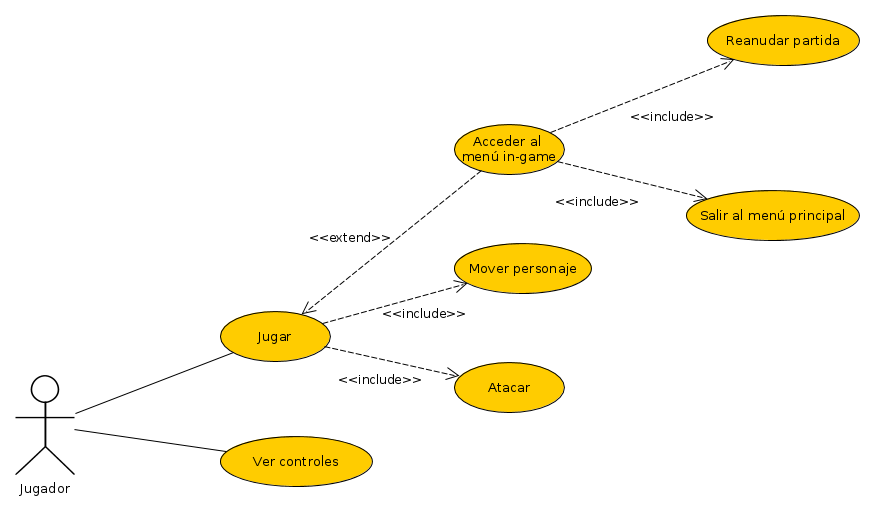
\includegraphics[width=.7\textwidth]{capitulos/diagramas/casos_uso_2.png}
	\caption{Diagrama de casos de uso.}\label{fig:casos_uso}
\end{figure}
\FloatBarrier{}

Dado que el procesamiento del juego transcurre de forma local en la consola, mediante un dispositivo único, solo existe un actor en el sistema y por ende, un perfil de usuario. \\ \\

\begin{table}[h]
	\centering
	\begin{tabular}{| l | p{10cm} |}
		\hline
		\textbf{PU-1} & \textbf{Jugador}  \\ \hline
		Descripción & Perfil utilizado para identificar cualquier usuario que juegue al producto desarrollado, tanto en emuladores como en hardware.  \\ \hline
		Actores asociados & ACT-1 (Jugador) \\ \hline
		Comentarios & Ninguno.  \\ \hline
	\end{tabular}
	\caption{Perfil de Usuario 1.}\label{tab:pu-1}
\end{table}

\begin{table}[h]
	\centering
	\begin{tabular}{| l | p{10cm} |}
		\hline
		\textbf{ACT-1} & \textbf{Jugador}  \\ \hline
		Perfil de usuario & PU-1 \\ \hline
		Requisitos asociados & RF-1, RF-2, RF-3, RF-4, RF-5, RF-6, RF-7 \\ \hline
		Descripción & Formado por la persona que juega y utiliza el software desarrollado. \\ \hline
		Comentarios & Ninguno.  \\ \hline
	\end{tabular}
	\caption{Actor 1.}\label{tab:act-1}
\end{table}
\FloatBarrier{}

\subsection{Requisitos funcionales}
En esta sección se incluirán los requisitos funcionales del proyecto, extraídos del diagrama de casos de uso.

%\multicolumn{2}{c|}

\begin{table}[h]
	\centering
	\begin{tabular}{| l | p{11cm} |}
		\hline
		\textbf{RF-1} & \textbf{Jugar} \\ \hline
		Objetivos asociados & OBJ-1, OBJ-2, OBJ-3, OBJ-4 \\ \hline
		Requisitos asociados & RI-1 \\ \hline
		Descripción & El jugador inicia la partida. \\ \hline
		Precondición & El jugador debe haber encontrarse en el menú principal.  \\ \hline
		Secuencia normal & 
		\begin{enumerate}
			\item Mover el cursor al botón adecuado.
			\item El jugador presiona ``A''.
			\item Se carga el último nivel que no haya sido superado.
		\end{enumerate}
		\\ \hline
		Postcondición & El jugador inicia una partida. \\ \hline
		Excepciones & Ninguna. \\ \hline
		Comentarios & Ninguno. \\ \hline
	\end{tabular}
	\caption{Requisito funcional 1.}\label{tab:rf-1}
\end{table}

\begin{table}[h]
	\centering
	\begin{tabular}{| l | p{11cm} |}
		\hline
		\textbf{RF-2} & \textbf{Ver controles} \\ \hline
		Objetivos asociados & OBJ-1 \\ \hline
		Requisitos asociados & Ninguno. \\ \hline
		Descripción & El jugador selecciona la visualización de los controles. \\ \hline
		Precondición & El jugador debe haber encontrarse en el menú principal.  \\ \hline
		Secuencia normal & 
		\begin{enumerate}
			\item Mover el cursor al botón adecuado.
			\item El jugador presiona ``A''.
			\item El juego carga los nombres por pantalla.
		\end{enumerate}
		\\ \hline
		Postcondición & El jugador visualiza los controles por pantalla. \\ \hline
		Excepciones & Ninguna. \\ \hline
		Comentarios & Ninguno. \\ \hline
	\end{tabular}
	\caption{Requisito funcional 2.}\label{tab:rf-2}
\end{table}

\begin{table}[h]
	\centering
	\begin{tabular}{| l | p{11cm} |}
		\hline
		\textbf{RF-3} & \textbf{Acceder al menú in-game} \\ \hline
		Objetivos asociados & OBJ-1 \\ \hline
		Requisitos asociados & Ninguno. \\ \hline
		Descripción & El jugador accede al menú del juego. Desde ahí puede seleccionar varias opciones \\ \hline
		Precondición & El jugador debe encontrarse en mitad de una partida.  \\ \hline
		Secuencia normal & 
		\begin{enumerate}
			\item El jugador presiona ``Start''.
			\item El juego carga un menú sobre la partida actual.
		\end{enumerate}
		\\ \hline
		Postcondición & El jugador visualiza los un menú. \\ \hline
		Excepciones & Ninguna. \\ \hline
		Comentarios & Las físicas del juego se ven pausadas ya que la ``delta'' del juego no se actualiza. \\ \hline
	\end{tabular}
	\caption{Requisito funcional 3.}\label{tab:rf-3}
\end{table}

\begin{table}[h]
	\centering
	\begin{tabular}{| l | p{11cm} |}
		\hline
		\textbf{RF-4} & \textbf{Mover personaje} \\ \hline
		Objetivos asociados & OBJ-1, OBJ-4 \\ \hline
		Requisitos asociados & Ninguno. \\ \hline
		Descripción & El jugador mueve el personaje principal. \\ \hline
		Precondición & El jugador debe encontrarse en mitad de una partida.  \\ \hline
		Secuencia normal & 
		\begin{enumerate}
			\item El jugador presiona cualquiera de los que habilitan el movimiento del personaje.
			\item El juego actualiza la posición del personaje según la entrada del jugador.
			\item El juego comprueba cualquier tipo de colisión para actualizar el estado del jugador o sobrescribir la posición del mismo.
		\end{enumerate}
		\\ \hline
		Postcondición & El personaje ve actualizada su posición y estado. \\ \hline
		Excepciones & Ninguna. \\ \hline
		Comentarios & Ninguno. \\ \hline
	\end{tabular}
	\caption{Requisito funcional 4.}\label{tab:rf-4}
\end{table}

\begin{table}[h]
	\centering
	\begin{tabular}{| l | p{11cm} |}
		\hline
		\textbf{RF-5} & \textbf{Atacar} \\ \hline
		Objetivos asociados & OBJ-1, OBJ-4 \\ \hline
		Requisitos asociados & Ninguno. \\ \hline
		Descripción & El jugador ataca. \\ \hline
		Precondición & El jugador debe encontrarse en mitad de una partida y el personaje no puede estar en el aire.  \\ \hline
		Secuencia normal & 
		\begin{enumerate}
			\item El jugador presiona ``B''.
			\item El juego comprueba si existe contacto con algún enemigo.
			\item En caso afirmativo, el juego procesa el ataque.
		\end{enumerate}
		\\ \hline
		Postcondición & En caso de contacto, los enemigos ven actualizado su estado. \\ \hline
		Excepciones & Ninguna. \\ \hline
		Comentarios & Ninguno. \\ \hline
	\end{tabular}
	\caption{Requisito funcional 5.}\label{tab:rf-5}
\end{table}

\begin{table}[h]
	\centering
	\begin{tabular}{| l | p{11cm} |}
		\hline
		\textbf{RF-6} & \textbf{Reanudar partida} \\ \hline
		Objetivos asociados & OBJ-1 \\ \hline
		Requisitos asociados & Ninguno. \\ \hline
		Descripción & El jugador reanuda la partida después de haber pausado el juego. \\ \hline
		Precondición & El jugador debe encontrarse en el menú in-game.  \\ \hline
		Secuencia normal & 
		\begin{enumerate}
			\item Mover el cursor al botón adecuado.
			\item El jugador presiona ``A''.
			\item El juego desocupa los recursos que utilizaba el menú in-game y reanuda la partida.
		\end{enumerate}
		\\ \hline
		Postcondición & La partida es reanudada y la ``delta'' vuelve a actualizarse. \\ \hline
		Excepciones & Ninguna. \\ \hline
		Comentarios & Ninguno. \\ \hline
	\end{tabular}
	\caption{Requisito funcional 6.}\label{tab:rf-6}
\end{table}
\FloatBarrier{}

\begin{table}[h]
	\centering
	\begin{tabular}{| l | p{11cm} |}
		\hline
		\textbf{RF-7} & \textbf{Salir al menú principal} \\ \hline
		Objetivos asociados & OBJ-1 \\ \hline
		Requisitos asociados & Ninguno. \\ \hline
		Descripción & El jugador vuelve al menú principal del juego. \\ \hline
		Precondición & El jugador debe encontrarse en el menú in-game.  \\ \hline
		Secuencia normal & 
		\begin{enumerate}
			\item Mover el cursor al botón adecuado.
			\item El jugador presiona ``A''.
			\item El juego desocupa los recursos que utilizaba el nivel del juego y carga el menú principal.
		\end{enumerate}
		\\ \hline
		Postcondición & El juego carga el menú principal. \\ \hline
		Excepciones & Ninguna. \\ \hline
		Comentarios & Ninguno. \\ \hline
	\end{tabular}
	\caption{Requisito funcional 7.}\label{tab:rf-7}
\end{table}

\subsection{Requisitos de información}
En esta sección se incluirán los requisitos de información del proyecto. Esto solo involucra el progreso que ha hecho el jugador en previas sesiones de juego.

\vspace{2cm}

\begin{table}[h]
	\centering
	\begin{tabular}{| l | p{11cm} |}
		\hline
		\textbf{RI-1} & \textbf{``Save file''} \\ \hline
		Objetivos asociados & OBJ-5 \\ \hline
		Requisitos asociados & Ninguno. \\ \hline
		Descripción & El juego debe almacenar el progreso realizado por el jugador. \\ \hline
		Datos específicos & 
		\begin{itemize}
			\item Último nivel completado: Número entero.
		\end{itemize}
		\\ \hline
		Comentarios & Ninguno. \\ \hline
	\end{tabular}
	\caption{Requisito de información 1.}\label{tab:ri-1}
\end{table}
\FloatBarrier{}
\newpage
\subsection{Requisitos no funcionales}
En esta sección se incluirán los requisitos no funcionales del proyecto.

\vspace{2cm}

\begin{table}[h]
	\centering
	\begin{tabular}{| l | p{11cm} |}
		\hline
		\textbf{RNF-1} & \textbf{Rendimiento} \\ \hline
		Objetivos asociados & OBJ-1, OBJ-2, OBJ-3, OBJ-4 \\ \hline
		Requisitos asociados & Ninguno. \\ \hline
		Descripción & Con la finalidad de ofrecer una experiencia jugable agradable al jugador, el juego tiene como objetivo ofrecer una tasa de refresco de 60 fotogramas por segundo. Para ello se utiliza en la medida de lo posible cualquier opción que acelere el procesamiento del juego por medio de hardware. \\ \hline
		Comentarios & En el caso del proyecto, se ha optado por utilizar tiles y sprites antes que el modo bitmap. También se debe tener en cuenta las limitaciones y ventajas que ofrece el hardware del dispositivo, un ejemplo de ello es utilizar en la medida de lo posible enteros de 32 bits como tipo de datos o evitar hacer escrituras de 1 byte en la VRAM. \\ \hline
	\end{tabular}
	\caption{Requisito no funcional 1.}\label{tab:rnf-1}
\end{table}

\vspace{2cm}

\begin{table}[h]
	\centering
	\begin{tabular}{| l | p{11cm} |}
		\hline
		\textbf{RNF-2} & \textbf{Batería} \\ \hline
		Objetivos asociados & OBJ-1, OBJ-2, OBJ-3, OBJ-4 \\ \hline
		Requisitos asociados & Ninguno. \\ \hline
		Descripción & El juego además de tener que ofrecer un buen rendimiento, debe tener como prioridad maximizar el uso de la batería cuando sea posible. \\ \hline
		Comentarios & De manera simplificada, el objetivo es hacer que el procesador se encuentre el máximo tiempo posible en un estado de baja energía (mediante el uso de interrupciones por ejemplo). \\ \hline
	\end{tabular}
	\caption{Requisito no funcional 2.}\label{tab:rnf-2}
\end{table}

\begin{table}[h]
	\centering
	\begin{tabular}{| l | p{11cm} |}
		\hline
		\textbf{RNF-3} & \textbf{Accesibilidad y usabilidad} \\ \hline
		Objetivos asociados & OBJ-1 \\ \hline
		Requisitos asociados & Ninguno. \\ \hline
		Descripción & El producto desarrollado debe ofrecer una experiencia familiar y similar, en cuánto a controles se refiere, a otros juegos. Además, la estética y temática debe ser aceptable para cualquier tipo de público independientemente de la edad. \\ \hline
		Comentarios & Dado que el juego tiene que proporcionar una experiencia aceptable para cualquier tipo de público independientemente de la edad, se ha optado por ofrecer una experiencia similar a lo que describe la calificación PEGI 3\tablefootnote{https://pegi.info/what-do-the-labels-mean}. \\ \hline
	\end{tabular}
	\caption{Requisito no funcional 3.}\label{tab:rnf-3}
\end{table}

\begin{table}[h]
	\centering
	\begin{tabular}{| l | p{11cm} |}
		\hline
		\textbf{RNF-4} & \textbf{Mantenibilidad} \\ \hline
		Objetivos asociados & OBJ-1, OBJ-2, OBJ-3, OBJ-4, OBJ-5 \\ \hline
		Requisitos asociados & Ninguno. \\ \hline
		Descripción & Facilitar la comprensión, y posible contribución en un futuro, de personas ajenas al desarrollo inicial del juego. \\ \hline
		Comentarios & El desarrollo del código se llevará a cabo acorde con las pautas marcadas por el \textit{Linux kernel coding style} elaborado por el equipo de desarrollo del kernel Linux. \\ \hline
	\end{tabular}
	\caption{Requisito no funcional 4.}\label{tab:rnf-4}
\end{table}
\FloatBarrier{}

\begin{table}[h]
	\centering
	\begin{tabular}{| l | p{11cm} |}
		\hline
		\textbf{RNF-5} & \textbf{Administración del progreso del jugador} \\ \hline
		Objetivos asociados & OBJ-5 \\ \hline
		Requisitos asociados & RI-1 \\ \hline
		Descripción & Crear una experiencia de juego continua, sin cortes, donde el progreso del jugador se guardará sin que este tenga que manualmente especificarlo. \\ \hline
		Comentarios & El progreso del jugador solo se verá actualizado cuando este supere un nivel que no haya superado anteriormente. \\ \hline
	\end{tabular}
	\caption{Requisito no funcional 5.}\label{tab:rnf-5}
\end{table}

\section{Desarrollo}\label{sec:aspectos}
Una vez comentadas las especificaciones del proyecto, se dedica esta sección a comentar el funcionamiento específico de varias partes del código. Para una visión general del código se ha optado por utilizar diagramas de flujo, mientras que para una descripción específica del código se ha optado por utilizar pseudocódigo. Además, se comentarán aspectos destacables del desarrollo realizado. La estructura general se inspira en~\cite{bib:ing_vid}. 

\subsection{Menú}
El diagrama de flujo del menú se puede observar en la Figura~\ref{fig:flujo_menu}, siendo lo único destacable del proceso el procesamiento de la entrada del usuario.

Una vez transicionado del inicio a la escena donde se muestra el menú del juego, se cargan los \textit{assets} que se utilizarán para el menú principal y se lee cualquier dato guardado de partidas previas. Posteriormente, en un bucle infinito, se procede a actualizar las animaciones y posiciones de los \textit{sprites} y fondos del menú (el menú es dinámico). En cada iteración del bucle, se consulta el ``input'' del usuario y en caso de no reconocer el botón presionado como válido se vuelve al inicio del bucle, actualizando los elementos que no controla el jugador y esperando a que se acabe de renderizar el fotograma actual.

En caso de ser válido, se comprueba si el ``input'' mueve el cursor o presiona el botón seleccionado. En caso de mover el cursor, se actualiza la posición del \textit{sprite}. En caso de presionar el botón seleccionado, se cargará la siguiente escena. 

\begin{figure}[h]
	\centering
	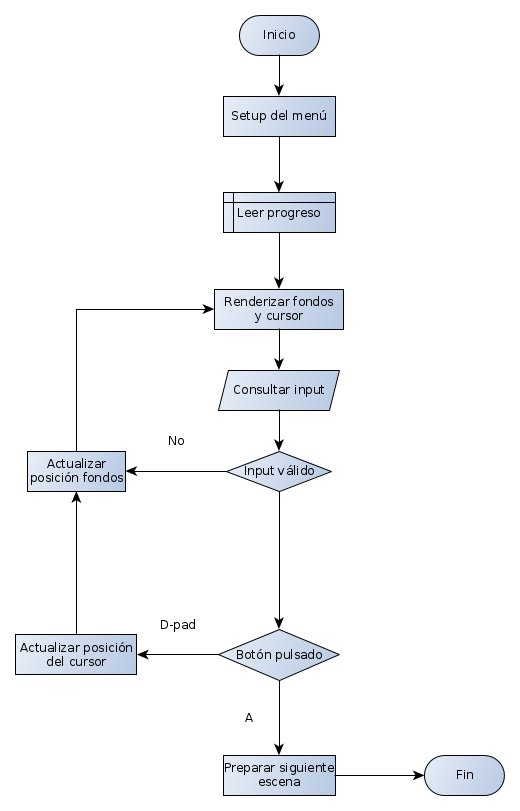
\includegraphics[width=.5\textwidth]{capitulos/diagramas/flujo_menu.png}
	\caption{Diagrama de flujo del menú principal.}\label{fig:flujo_menu}
\end{figure}
\FloatBarrier{}

\subsection{Nivel del juego}
Para cada nivel del juego, se lee la entrada del usuario y se procesa de forma acorde, además de actualizar de forma independiente los enemigos y objetos del nivel. El proceso se puede observar en la Figura~\ref{fig:flujo_nivel}.

\begin{figure}[h]
	\centering
	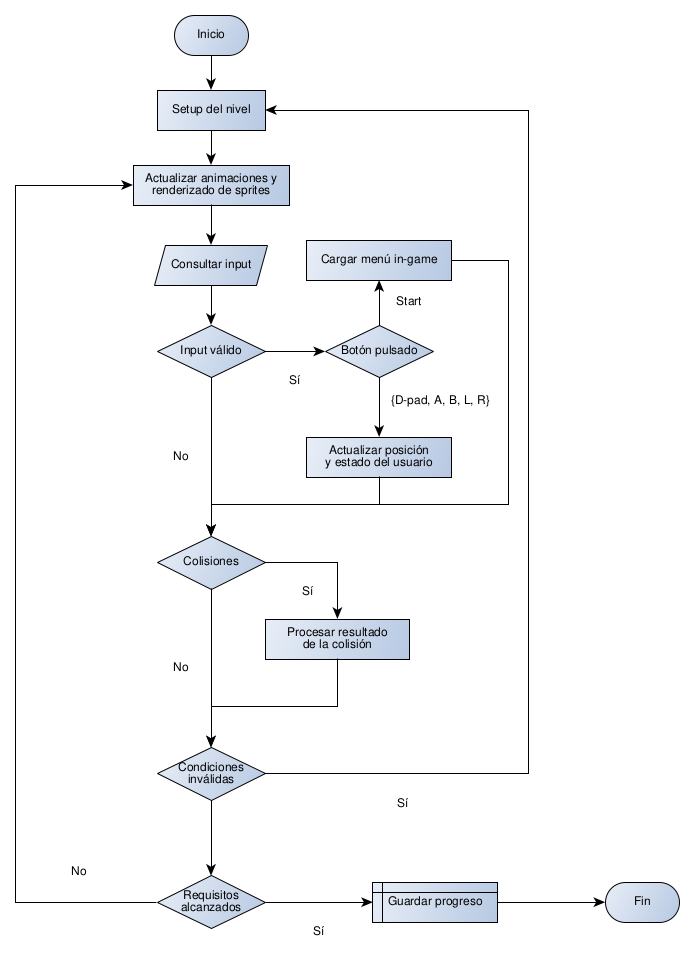
\includegraphics[width=.65\textwidth]{capitulos/diagramas/flujo_nivel.png}
	\caption{Diagrama de flujo para cada nivel del juego.}\label{fig:flujo_nivel}
\end{figure}
\FloatBarrier{}

A diferencia del menú, el cual no contaba con enemigos, en el bloque de ``Actualizar animaciones y renderizado de sprites'' también se actualizan las posiciones de enemigos y objetos que puedan aparecer en el nivel. De forma adicional, se dedica un bloque al procesamiento de colisiones en los que se tiene en cuenta el entorno y otras entidades. Dado que para completar el nivel se tienen que cumplir ciertas condiciones, al final de cada iteración del bucle se comprueba si las condiciones se han cumplido y si el jugador debe reiniciar el nivel actual o pasar al siguiente. Es importante recalcar que el jugador no puede guardar manualmente el progreso, este solo se puede guardar en caso de que el jugador consiga pasar al siguiente nivel.

También, como se hizo referencia en el diagrama de casos de uso, se permite acceder a un menú in-game. El proceso es similar al visto en menú principal pero con ligeros cambios tal y como se puede observar en la Figura~\ref{fig:flujo_ingame}.


\begin{figure}[h]
	\centering
	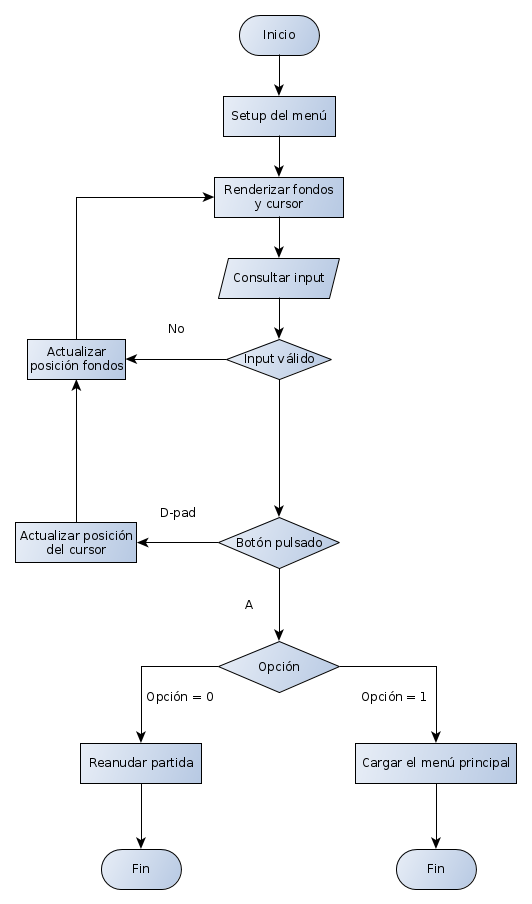
\includegraphics[width=.5\textwidth]{capitulos/diagramas/flujo_ingame.png}
	\caption{Diagrama de flujo para el menú in-game.}\label{fig:flujo_ingame}
\end{figure}
\FloatBarrier{}

El bloque de ``Colisiones'', mostrado en la Figura~\ref{fig:flujo_nivel}, sigue los pasos mostrados a continuación para procesar las colisiones del juego:

\begin{itemize}
	\item Comprueba las colisiones del entorno en el eje X del personaje principal.
	\item Comprueba las colisiones del entorno en el eje Y del personaje principal.
	\item Comprueba las colisiones del entorno en el eje X de los enemigos.
	\item Comprueba las colisiones entre los enemigos y el personaje principal.
\end{itemize}

A continuación, se mostrará el pseudocódigo de cada uno de los apartados que conforma el bloque de ``Colisiones''. Las funciones mostradas (Algoritmos~\ref{algo:col_entorno_x} y~\ref{algo:col_entorno_y}) se han simplificado, omitiendo el procesamiento necesario al trabajar con valores desplazados por 8 bits (representación de coma fija).

Sin embargo, antes de mostrar el pseudocódigo destinado a las colisiones, se muestra el Listado~\ref{lst:se_index}, utilizada para conseguir el índice de un \textit{tile} específico. La función no sigue el cálculo habitual de $x+y*w$\footnote{Los fondos que utilizan la matriz de transformación si siguen la ecuación convencional, pero para el proyecto se utilizarán fondos ``normales'', en los cuales hay que seguir la metodología mostrada.} por culpa de la distribución no uniforme de los \textit{tiles} en la VRAM~\cite{bib:tonc}.

\vspace{1cm}

\begin{lstlisting}[language=c,label=lst:se_index,caption=Fragmento de código de la librería TONC.]
uint32_t se_index(uint32_t y, uint32_t x)
{
	// n = x + y * 32
	uint32_t n = x + (y << 5);

	if(x >= 32) {
		n += 0x03E0;
	}

	if(y >= 32 && IS_BG_512x512) {
		n += 0x0400;
	}

	return n;
}
\end{lstlisting}

\vspace{2cm}

\begin{algorithm}[h]
	\SetAlgorithmName{Algoritmo}{}
	\footnotesize
	\caption{Procesa el incremento en el eje X teniendo en cuenta el entorno.}
	\label{algo:col_entorno_x}
	\DontPrintSemicolon % Some LaTeX compilers require you to use \dontprintsemicolon instead
	\KwIn{y, x, incremento}
	\KwOut{incremento}

	\tcp{Si se mueve a la derecha, se añade un offset}
	\If{$incremento > 0$} {
		$x \gets x + offset$\;
	}

	\tcp{Cada tile ocupa 8 píxeles}
	$incTiles \gets abs(incremento) / 8$\;
	\tcp{Se recorre cada tile recorrido con el incremento}
	\For{$i \gets 0$ \textbf{to} $incTiles$} {
		\tcp{Se recorre el espacio que ocupa la altura del personaje}
		\For{$j \gets 0$ \textbf{to} $alturaPersonaje$} {
			\tcp{Se suma i en caso de ir a la derecha}
			\tcp{y se resta en caso de ir a la izquierda}
			$tile \gets getTileMapa(y+j, x{\pm}i)$\;
			\If{$tile\;es\;prohibido$} {
				$incremento \gets maxIncPermitido(x,i)$\;
				\Return{$incremento$}\;
			}
		}
		}
		\Return{$incremento$}\;
\end{algorithm}

\begin{algorithm}[h]
	\SetAlgorithmName{Algoritmo}{}
	\footnotesize
	\caption{Procesa el incremento en el eje Y teniendo en cuenta el entorno.}
	\label{algo:col_entorno_y}
	\DontPrintSemicolon % Some LaTeX compilers require you to use \dontprintsemicolon instead
	\KwIn{y, x, incremento}
	\KwOut{incremento}

	\tcp{Si se mueve hacia abajo, se añade un offset}
	\If{$incremento > 0$} {
		$y \gets y + offset$\;
	}

	\tcp{Cada tile ocupa 8 píxeles}
	$incTiles \gets abs(incremento) / 8$\;
	\tcp{Se recorre cada tile recorrido con el incremento}
	\For{$i \gets 0$ \textbf{to} $incTiles$} {
		\tcp{Se recorre el espacio que ocupa la anchura del personaje}
		\For{$j \gets 0$ \textbf{to} $anchuraPersonaje$} {
			\tcp{Se suma i en caso de ir abajo}
			\tcp{y se resta en caso de ir arriba}
			$tile \gets getTileMapa(y{\pm}i, x+j)$\;
			\If{$tile\;es\;prohibido$} {
				$incremento \gets maxIncPermitido(y,i)$\;
				\Return{$incremento$}\;
			}
		}
		}
		\Return{$incremento$}\;
\end{algorithm}
\FloatBarrier{}

En el caso de los enemigos, la dirección en la que se mueven se ve afectada por las colisiones que detecten. En caso de colisionar, el enemigo se invertirá y moverá en la dirección contraria. Por razones de optimización se omiten:

\begin{itemize}
	\item La comprobación del eje Y dado que los enemigos no pueden saltar. Para comprobar si los enemigos se acercan a una posición en caída libre, se comprobará el \textit{tile} posicionado debajo. De ahí el $alturaEnemigo+1$.
	\item El cálculo del mayor incremento permitido dado que no afectará de forma considerable la jugabilidad. Esta es la razón por la que se retorna 0 dentro del bucle.
\end{itemize}

A diferencia del movimiento del personaje, el movimiento de los enemigos se realiza de forma independiente. En cada iteración se llamará a un método que recorrerá todos los enemigos vivos para actualizar su posición utilizando el Algoritmo~\ref{algo:pos_enemigo}. Es necesario aclarar el uso del parámetro $a$, valor que será diferente dependiendo del enemigo. Si el movimiento del enemigo no permite el movimiento por ``aire'', el parámetro $a$ será mayor o igual a 1. En caso de que el movimiento del personaje permita desplazarse sin tener ningún bloque sólido debajo, el valor del parámetro $a$ será 0.

\begin{algorithm}[h]
	\SetAlgorithmName{Algoritmo}{}
	\footnotesize
	\caption{Procesa el incremento en el eje X del enemigo teniendo en cuenta el entorno.}
	\label{algo:pos_enemigo}
	\DontPrintSemicolon % Some LaTeX compilers require you to use \dontprintsemicolon instead
	\KwIn{y, x, incremento}
	\KwOut{incremento}

	\tcp{Si se mueve a la derecha, se añade un offset}
	\If{$incremento > 0$} {
		$x \gets x + offset$\;
	}

	\tcp{Cada tile ocupa 8 píxeles}
	$incTiles \gets abs(incremento) / 8$\;
	\tcp{Se recorre cada tile recorrido con el incremento}
	\For{$i \gets 0$ \textbf{to} $incTiles$} {
		\tcp{Se recorre el espacio que ocupa la altura del enemigo + a}
		\tcp{a denota si el enemigo procesará los bloques que estén debajo}
		\For{$j \gets 0$ \textbf{to} $alturaEnemigo+a$} {
			\tcp{Se suma i en caso de ir a la derecha}
			\tcp{y se resta en caso de ir a la izquierda}
			$tile \gets getTileMapa(y+j, x{\pm}i)$\;
			\If{$tile\;es\;prohibido$} {
				\Return{$0$}\;
			}
		}
		}
		\Return{$incremento$}\;
\end{algorithm}

Finalmente, la detección de colisiones entre el personaje principal y los enemigos se realiza tal y como se muestra en el Algoritmo~\ref{algo:collisions}.

\begin{algorithm}[h]
	\SetAlgorithmName{Algoritmo}{}
	\footnotesize
	\caption{Procesa las colisiones entre los enemigos y el personaje.}
	\label{algo:collisions}
	\DontPrintSemicolon % Some LaTeX compilers require you to use \dontprintsemicolon instead
	\KwIn{numeroEnemigos}

	\If{$personaje.estado\;esta\;siendo\;atacado$} {
		\Return{}\;
	}

	\tcp{Se recorren todos los enemigos vivos}
	\For{$i \gets 0$ \textbf{to} $numeroEnemigos$} {
		\tcp{Si la distancia entre las dos entidades es menor}
		\tcp{que la distancia minima declarada para el eje Y}
		\tcp{continuar comprobando el eje X}
		\If{$abs(personaje.y - enemigos[i].y) < distColisionY$} {
			\If{$abs(personaje.x - enemigos[i].x) < distColisionX$} {
				$personaje.estado \gets ATACADO$\;
				$personaje.vida \gets personaje.vida - 1$\;
			}
			$posicionEspada \gets personaje.x \pm offset$\;
			\If{$atacando \And abs(posicionEspada-enemigos[i].x) < distColisionX$} {
				$enemigos.vida \gets enemigos.vida - 1$\;
			}
		}
	}
\end{algorithm}
\FloatBarrier{}

\section{Aspectos destacados del desarrollo}
En esta sección, se comentan los aspectos a tener en cuenta del desarrollo y algunas de las prácticas y conocimientos obtenidos en la tarea de ``Estudio de las técnicas de programación'' programada en la planificación del proyecto.

\subsection{Pruebas de rendimiento}
La GBA no es un sistema convencional dado que no tiene una forma de mostrar información fácilmente por pantalla. Es por esto, que para las pruebas de rendimiento realizadas se ha utilizado un sistema peculiar. Entre las formas que se han utilizado para medir el rendimiento se distinguen:

\begin{itemize}
	\item Medida que incluye No\$GBA en su interfaz para comprobar rápidamente la carga de la CPU (véase la Figura~\ref{fig:nogba_bench}). A pesar de ser un medio poco fiable, es de utilidad para hacerse una idea general del rendimiento, y para distinguir de inmediato rutinas con una amplia diferencia de rendimiento.

		\begin{figure}[h]
			\centering
			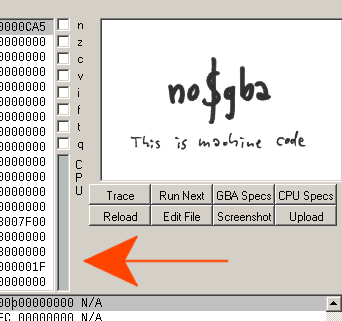
\includegraphics[width=.5\textwidth]{capitulos/capitulo5/nogba_bench.png}
			\caption{Interfaz que utiliza No\$GBA para mostrar el uso de la CPU.}\label{fig:nogba_bench}
		\end{figure}
		\FloatBarrier{}

	\item Uso de los temporizadores que incluye la consola para medir con más precisión. La visualización de los valores puede consultarse en el depurador o por pantalla. Dado que las pruebas se realizan también en hardware, se ha optado por mostrar los valores por pantalla dado que no se cuenta con el hardware necesario para mantener una conexión JTAG (véase la Figura~\ref{fig:bench_value}).

		\begin{figure}[h]
			\centering
			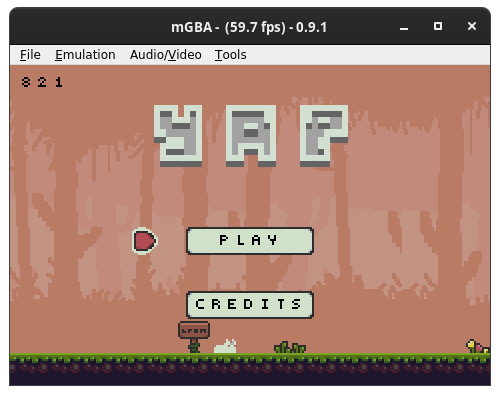
\includegraphics[width=.6\textwidth]{capitulos/capitulo5/bench_value.png}
			\caption{El valor del temporizador en la esquina superior izquierda.}\label{fig:bench_value}
		\end{figure}
		\FloatBarrier{}

		Un ejemplo donde se comparó la eficiencia de dos fragmentos de código, fue en la carga de \textit{assets} antes de iniciar una escena en el juego. Para la prueba se comparó el tiempo que transcurría al copiar los datos utilizando \textit{DMA} y la función \textit{memcpy}. El código utilizado es similar al mostrado en el Listado~\ref{lst:benchmark}.

		\vspace{1cm}

	\begin{lstlisting}[language=c,caption={Tomando medidas mediante temporizadores.},label={lst:benchmark}]

	// Se activa el temporizador a f = 262.21 KHz
	*((volatile uint16_t*)0x04000102) = 0x0081;

	// Se copian los datos ...

	// Se consigue el valor del temporizador
	timer = *((volatile uint16_t*)0x04000100);

	// Se desactiva el temporizador
	*((volatile uint16_t*)0x04000102) = 0x0000;

	// Se muestra el valor por pantalla ...

	\end{lstlisting}

		Con los valores del \textit{benchmark} obtenidos, se divide la frecuencia utilizada entre el temporizador para hallar los segundos que han transcurrido. En el caso del ejemplo anterior los resultados se muestran en la Figura~\ref{fig:plot_bench}. Con estos resultados se llegó a la conclusión de cargar los datos mediante \textit{DMA} era la opción más adecuada. 

		\begin{figure}[h]
			\centering
			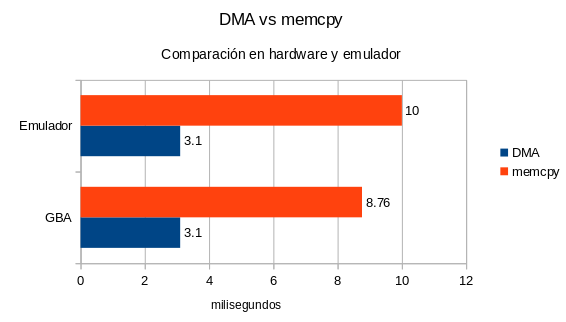
\includegraphics[width=.55\textwidth]{capitulos/capitulo5/graph_bench.png}
			\caption{Resultados de la prueba de rendimiento.}\label{fig:plot_bench}
		\end{figure}
\end{itemize}
\FloatBarrier{}

\subsection{Sincronización vertical}
Uno de los primeros problemas que surgieron en el desarrollo del juego, fue la desincronización vertical que se producía al actualizar los fondos y~\textit{sprites} por pantalla. Este fenómeno se produce cuando se actualizan objetos mientras la pantalla se está actualizando. Una instancia donde se puede observar este problema se muestra en la Figura~\ref{fig:torn}, en concreto en la parte superior de la imagen. Aquí, se puede observar la distorsión que se produce en el personaje y la moneda. 

\begin{figure}[h]
	\centering
	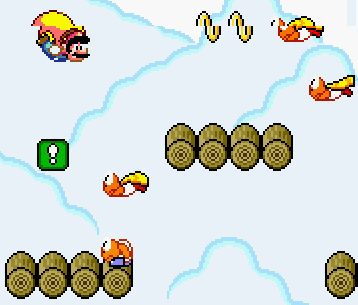
\includegraphics[width=.4\textwidth]{capitulos/capitulo5/torn.png}
	\caption[Desincronización vertical.]{Desincronización vertical. Imagen obtenida de \cite{bib:washington}.}\label{fig:torn}
\end{figure}
\FloatBarrier{}

Inicialmente para resolver el problema, el programa se esperaba a que la consola terminase de renderizar el fotograma actual para cambiar las posiciones de los fondos y objetos. Para ello se comprueba el valor de VCount en la dirección de memoria 0x04000006 mediante dos bucles \textit{while} mostrados en el Listado~\ref{lst:vsync_1}~\cite{bib:tonc}. La finalidad del primer bucle es la de evitar actualizar el fotograma más de una vez cuando el procesamiento realizado se completa antes de renderizarse el siguiente fotograma.

\begin{lstlisting}[language=c,caption={Implementación de VSync mediante dos bucles.},label={lst:vsync_1}]
volatile uint16_t *vcount = (volatile uint16_t*)0x04000006;

while (*vcount >= 160);
while (*vcount < 160);

// Actualizar posiciones y estados ...
\end{lstlisting}

Sin embargo, esta implementación no es eficiente y no cumple con los requisitos no funcionales RNF-1 y RNF-2, dado que el procesador se encuentra al 100\% mientras espera para procesar el siguiente fotograma. La solución por lo tanto, es utilizar las interrupciones del sistema, evitando así un consumo excesivo del procesador y de la batería. Esto se consigue, con la instrucción de ensamblador \textit{swi}, la cual en la Game Boy Advance llamará a una de las funciones predefinidas de la BIOS. En este caso, la función que interesa utilizar es la 0x05, la función que pone al dispositivo en un estado de baja energía hasta que se produzca una interrupción VBlank. Para más información sobre las funciones disponibles consultar el Apéndice~\ref{ap:bios}.

Al abrir uno de los prototipos en el emulador No\$GBA, el cual ofrece una gráfica mostrando el uso del procesador, se puede observar una importante diferencia en consumo. En la Figura~\ref{fig:vsync_irq} se observa a la izquierda, el procesador al 100\% sin que ninguno de los personajes se mueva, mientras que a la derecha se observa un uso de la CPU casi inexistente al utilizar interrupciones.

\begin{figure}[h]
	\centering
	\begin{subfigure}[b]{0.45\textwidth}
		\centering
		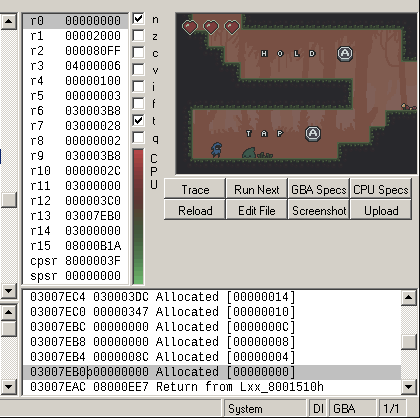
\includegraphics[width=\textwidth]{capitulos/capitulo5/wout_irq.png}
		\label{fig:wout_irq}
		\caption{Rendimiento sin utilizar interrupciones.}
	\end{subfigure}
	\hfill
	\begin{subfigure}[b]{0.45\textwidth}
		\centering
		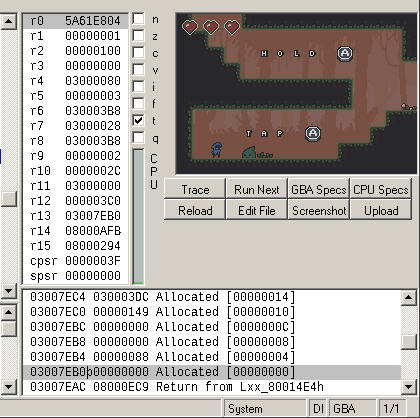
\includegraphics[width=\textwidth]{capitulos/capitulo5/with_irq.png}
		\label{fig:with_irq}
		\caption{Rendimiento utilizando interrupciones.}
	\end{subfigure}
	\caption{Rendimiento de las dos alternativas disponibles.}
	\label{fig:vsync_irq}
\end{figure}

\subsection{Operaciones de punto flotante}
Una limitación importante que se tuvo en cuenta en el desarrollo fue el rendimiento de la consola al operar números de coma flotante, y dividir y realizar operaciones de módulo. Esto se debe a la falta de una \textit{FPU} (Unidad de Punto Flotante) y una implementación por hardware de la división en la consola \cite{bib:tonc}. Para remediar estas limitaciones, se procura desplazar bits antes que realizar una división y utilizar números de coma fija. Es necesario mencionar que los compiladores optimizan automáticamente las divisiones en base 2, pero por razones de consistencia, en el código se utilizarán operaciones \textit{shift} incluso para las divisiones en base 2.

Una demostración de una operación con números representados con coma fija para la sentencia $\frac{1}{2}+\frac{1}{2}$, se observa en el Listado~\ref{lst:fixed_numbers}.

\begin{lstlisting}[language=c,caption={Ejemplo de un cálculo con números de coma fija.},label={lst:fixed_numbers}]
int a, b, c;
a = b = 1 << 8;

a = a >> 1;
b = b >> 1;

c = a + b;
c = c >> 8; // c = 1

\end{lstlisting}

A pesar de tener que realizar un preprocesamiento y postprocesamiento de los datos, sigue siendo más eficiente que realizar una división de coma flotante en un dispositivo sin \textit{FPU}.

\subsection{Limitaciones de lectura y escritura}
Otra limitación del hardware afecta las operaciones de escritura y lectura sobre ciertas direcciones de memoria. La más llamativa es la limitación de escritura de la VRAM, RAM de paleta y OAM. En estas tres secciones el programador no puede realizar escrituras de 1 byte. En el caso de tener que escribir 1 byte, se tiene que leer 2 bytes, sobrescribir el byte que se desea modificar y actualizar el valor.

Otro ejemplo, esta vez de lectura, se encuentra en la mayoría de registros I/O. Los espacios de memoria dedicados a modificar los \textit{offsets} de los fondos, se puede escribir pero no se puede leer los valores almacenados. Esta es la razón por la que se tienen que utilizar variables auxiliares al trabajar con ciertos registros de entrada y salida.

\subsection{Texto}
Las dos opciones que se barajaron para mostrar texto por pantalla en el juego fueron una implementación por \textit{sprites} y una implementación por mapa. La primera consiste en reservar un espacio de la OAM y representar cada letra mediante un \textit{sprite} diferente. La segunda implementación, consiste en incluir el texto en los fondos, incluyendo cada una de las letras en los \textit{tiles}.

La implementación por la optó el autor fue una híbrida. Para los créditos iniciales, menú principal, menú de controles y menú in-game se utilizó una implementación mediante \textit{sprites}. Esto permitía al programador modificar fácilmente el texto mostrado por pantalla. Por otro lado, para los niveles, en concreto las indicaciones mostradas en los niveles, se utilizó una implementación por mapa. De esta forma el programador no se tenía que preocupar de cambiar la posición del texto cuando el jugador se moviese por el nivel.

\subsection{Preparación de los archivos binarios}
Dada la gran cantidad de imágenes y archivos de audio utilizados, el autor utilizó Grit, SuperFamiconv y Audacity para convertir los archivos originales a un array de bytes con el que el programa pueda trabajar. Para las imágenes, se programó un \textit{script} de BASH que automatizase el proceso, creando un mapa para cada escena, un conjunto de \textit{tiles} para cada grupo de escenas y una paleta de colores a compartir entre todos los fondos. Un ejemplo de la salida generada se puede observar en la Figura~\ref{fig:script}. Los comandos ejecutados en el \textit{script} se pueden consultar en el Apéndice~\ref{ap:scripts}.

\begin{figure}[h]
	\centering
	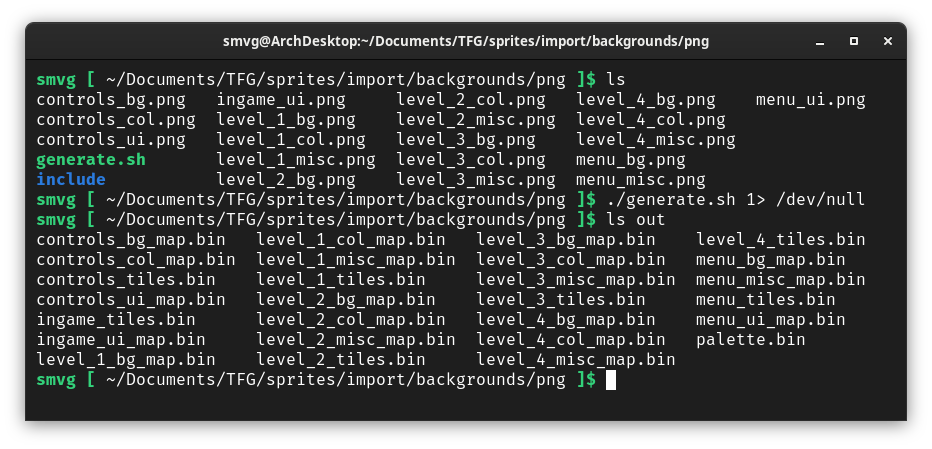
\includegraphics[width=.8\textwidth]{capitulos/capitulo5/salida_script.png}
	\caption{Archivos generados por el \textit{script}.}\label{fig:script}
\end{figure}
\FloatBarrier{}

En el caso de los archivos de audio, se utilizó Audacity para convertir todas las pistas de audio a un solo canal y a una frecuencia de 16 KHz. El resultado se exportaría después a un formato ``raw'' sin ningún tipo de cabecera~\cite{bib:washington}.

Con los archivos ``.bin'' generados, el siguiente paso es utilizarlos en el código, para ello el Makefile utilizado (y proporcionado por el \textit{toolchain}) para el proyecto incluye una regla para enlazar todos los archivos binarios al proyecto (véase la Figura~\ref{fig:makefile}). Esta regla permitirá al programador referenciar los archivos incluyendo en la cabecera un archivo con el siguiente formato: ``archivo\_bin.h'' siendo archivo el nombre del archivo utilizado sin contar la extensión. La variable que guarda el valor del archivo y la variable que guarda el tamaño en bytes sigue un formato similar al de la cabecera: ``archivo\_bin'' y ``archivo\_bin\_size'' respectivamente.

\begin{figure}[h]
	\centering
	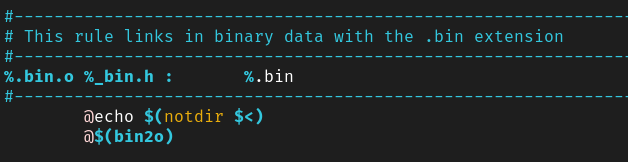
\includegraphics[width=.7\textwidth]{capitulos/capitulo5/makefile.png}
	\caption{Regla del Makefile.}\label{fig:makefile}
\end{figure}
\FloatBarrier{}
